\documentclass{article}
%\VignetteIndexEntry{KDETrees Simulation}
\usepackage{fullpage}
\title{KDETrees Simulations}
\author{Grady Weyenberg}
\usepackage{Sweave}
\begin{document}
\maketitle
\section{Introduction}
\label{sec:introduction}
Here we present the code for the simulations found in the KDETrees
article. These simulations compare the ability of KDETrees to find
trees which were generated by a non-contained coalescent process, in a
dataset consisting mostly of trees generated by a contained coalescent
process.
%% We test two scenarios: all contained coalescent trees are
%% contained in a single species tree; and the contained coalescent trees
%% are sampled from a mixed distribution, where the trees are contained
%% in one of 5 different species trees. We also compare the performance
%% of our method with that of the previously published Phylo-MCOA method.

The coalescent trees are generated using the methods found in the
Dendropy python module. The script which generates the trees, as well
as the species trees can be found in the {\tt sim} directory of the
KDETrees package.

\begin{Schunk}
\begin{Sinput}
> library(kdetrees)
> library(ape)
> library(ggplot2)
> library(parallel)
\end{Sinput}
\end{Schunk}

\section{Comparison of KDETrees and Phylo-MCOA}
\label{sec:comp-kdetr-phylo}
In this simulation we generate a test dataset which consists of one
``outlier'' tree, which is generated by an unconstrained coalescent
process, and 100 ``non-outlier'' trees which are generated by
constrained coalescent processes. The outlier trees used are those in
the {\tt species1.nex} file.
\begin{Schunk}
\begin{Sinput}
> out.trees <- unname(read.nexus("sim/species1k.nex"))
\end{Sinput}
\end{Schunk}
The non-outlier trees are created by the {\tt tresim.py} script.
This example call to the script will generate 100 coalescent trees
with effective population size 800 for each species tree found in
{\tt species.nex}.
\begin{Schunk}
\begin{Sinput}
> system2("sim/treesim.py",c("-s","sim/species.nex","-n",800,"-N",100))
\end{Sinput}
\end{Schunk}

First a wrapper to make mMCOA output resemble kdetrees output.
\begin{Schunk}
\begin{Sinput}
> source("sim/my-pmcoa.R")
> pmcoa <- function(trees,k=1.5,...){
+   list(i=which(detect.complete.outliers(pMCOA(trees,...),k=k)$TFgn))
+ }
\end{Sinput}
\end{Schunk}

Next a simulation function which generates a dataset and then
determines the false and true positive rates.
\begin{Schunk}
\begin{Sinput}
> sim <- function(neff,out.trees,sp.file="sim/species.nex",ncoal=100,...,f=kdetrees){
+   if(inherits(out.trees,"multiPhylo")) out.trees <- lapply(out.trees,c)
+   run <- function(otrees){
+     coaltrees <- read.tree(text=system2("sim/treesim.py", 
+                          c("-n",neff,"-s",sp.file,"-N",ncoal),stdout=TRUE))
+     res <- f(c(otrees,coaltrees),...)$i
+     hit <- sum(seq_along(otrees) %in% res)
+     c(hit=hit/length(otrees) , type1=(length(res)-hit)/length(coaltrees))
+   }
+   rowMeans(mcmapply(run,out.trees,SIMPLIFY=TRUE))
+ }
\end{Sinput}
\end{Schunk}

The ROC simulation varies the classification tuning parameter, $k$,
and tabulates FPR and TPR.
\begin{Schunk}
\begin{Sinput}
> roc.sim <- function(k,...){
+   foo <- function(kk,...) sim(...,k=kk)
+   res <- sapply(k,foo,...)
+   colnames(res) <- k
+   res
+ }
> #roc.sim(c(0,1,2),neff=2000,out.trees[1:10],f=pmcoa)
\end{Sinput}
\end{Schunk}

Simulation run. The effective population size of 2000 implies a
moderate amount of variance in the coalescent trees.
\begin{Schunk}
\begin{Sinput}
> options(mc.cores=4)
> k <- seq(-2,3,by=0.125)
> roc.kde <- roc.sim(k,neff=2000,out.trees[1:200], f=kdetrees)
> roc.kde.d <- roc.sim(k,neff=2000,out.trees[1:200], f=kdetrees,distance="d")
> roc.pmc <- roc.sim(k,neff=2000,out.trees[1:200], distance="p", f=pmcoa)
> save(roc.kde,roc.kde.d,roc.pmc,file="sim/rocsim.Rda")
\end{Sinput}
\end{Schunk}

\begin{Schunk}
\begin{Sinput}
> load("sim/rocsim.Rda")
> roc.df <- rbind(cbind(as.data.frame(t(roc.kde)),method="kde"),
+                 cbind(as.data.frame(t(roc.kde.d)),method="kdediss"),
+                 cbind(as.data.frame(t(roc.pmc)),method="pmcoa"))
> roc.plot <- ggplot(roc.df,aes(x=type1,y=hit,lty=method)) + geom_line() + xlim(0,1) + theme(legend.position="top") + labs(x="FPR",y="TPR")
> roc.plot
> ggsave("img/roc.pdf", width=4,height=3)
\end{Sinput}
\end{Schunk}

\begin{figure}
  \centering
  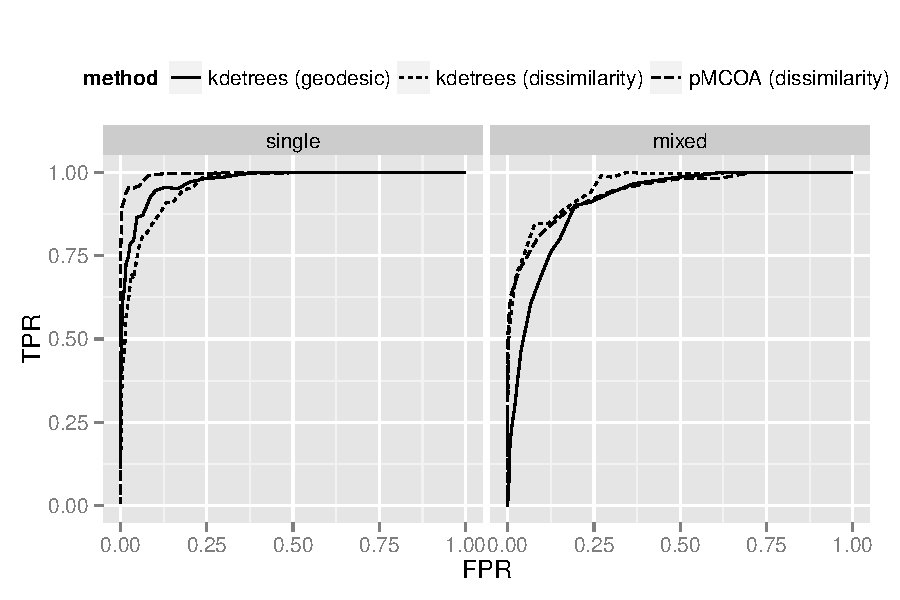
\includegraphics{img/rocmix.pdf}
  \caption{ROC curves comparing kdetrees and pMCOA as the
    classification tuning parameter is varied. Trees were generated
    from a coalescent distribution with $n_{eff}=2000$. kdetrees is
    run in geodesic distance with branch lengths mode, and pMCOA was
    run in "parastic" mode. (This seems the be best performing mode
    for each method in this scenario.)}
  \label{fig:roc}
\end{figure}


\begin{Schunk}
\begin{Sinput}
> roc.kde.mix <- roc.sim(k,neff=2000,out.trees[1:200], f=kdetrees,sp.file="sim/species5.nex",ncoal=20)
> roc.kde.mix.d <- roc.sim(k,neff=2000,out.trees[1:200], f=kdetrees,sp.file="sim/species5.nex",ncoal=20,distance="d")
> save(roc.kde.mix,roc.kde.mix.d,roc.pmc.mix,file="sim/rocmix.Rda")
\end{Sinput}
\end{Schunk}
\begin{Schunk}
\begin{Sinput}
> load("sim/rocmix.Rda")
> roc.df.mix <- rbind(cbind(as.data.frame(t(roc.kde.mix)),method="kde"), 
+                     cbind(as.data.frame(t(roc.kde.mix.d)),method="kdediss"),
+                     cbind(as.data.frame(t(roc.pmc.mix)),method="pmcoa"))
> rocdf <- rbind(cbind(roc.df,coal="single"),cbind(roc.df.mix,coal="mixed"))
> roc.mix.plot <- ggplot(rocdf,aes(x=type1,y=hit,lty=method)) + geom_line() + xlim(0,1) + theme(legend.position="top") + labs(x="FPR",y="TPR") + facet_grid(.~coal) + scale_linetype_discrete(labels=c("kdetrees (geodesic)","kdetrees (dissimilarity)","pMCOA (dissimilarity)"))
> roc.mix.plot
> ggsave("img/rocmix.pdf",width=6,height=4)
>  ##
> 
\end{Sinput}
\end{Schunk}

The next simulation looks at the TPR as we modify the variance of the
coalescent trees (neff parameter).
\begin{Schunk}
\begin{Sinput}
> neff.sim <- function(neff,...){
+   res <- sapply(neff, sim, ...)
+   colnames(res) <- neff
+   res
+ }
> #neff.sim(1000,out.trees[1:10],f=kdetrees)
\end{Sinput}
\end{Schunk}
\begin{Schunk}
\begin{Sinput}
> neff <- round(exp(seq(log(500),log(3000),len=10)))
> #### single
> tpr.kde <- neff.sim(neff,out.trees[1:200],f=kdetrees,k=0.751)
> tpr.kde.d <- neff.sim(neff,out.trees[1:200],f=kdetrees,k=1,distance="d")
> tpr.kde.t <- neff.sim(neff,out.trees[1:200],f=kdetrees,k=1,distance="d",topo.only=TRUE)
> tpr.pmc <- neff.sim(neff,out.trees[1:200],f=pmcoa,k=0.125)
> tpr.pmc.p <- neff.sim(neff,out.trees[1:200],f=pmcoa,k=0,distance="p")
> save(tpr.kde,tpr.pmc,tpr.kde.d,tpr.pmc.p,tpr.kde.t,file="sim/tprmix.Rda")
> #### mixed
> tpr.kde.mix <- neff.sim(neff,out.trees[1:200],f=kdetrees,k=0.7,sp.file="sim/species5.nex",ncoal=20)
> tpr.kde.d.mix <- neff.sim(neff,out.trees[1:200],f=kdetrees,k.65,distance="d",sp.file="sim/species5.nex",ncoal=20)
> tpr.kde.t.mix <- neff.sim(neff,out.trees[1:200],f=kdetrees,k=.7,distance="d",topo.only=TRUE,sp.file="sim/species5.nex",ncoal=20)
> tpr.pmc.mix <- neff.sim(neff,out.trees[1:200],f=pmcoa,k=0.25,sp.file="sim/species5.nex",ncoal=20)
> tpr.pmc.p.mix <- neff.sim(neff,out.trees[1:200],f=pmcoa,k=0.25,distance="p",sp.file="sim/species5.nex",ncoal=20)
> save(tpr.kde.mix,tpr.pmc.mix,tpr.kde.d.mix,tpr.pmc.p.mix,tpr.kde.t.mix,file="sim/tprmix.Rda")
> #### single default
> def.tpr.kde <- neff.sim(neff,out.trees[1:200],f=kdetrees)
> def.tpr.kde.d <- neff.sim(neff,out.trees[1:200],f=kdetrees,distance="d")
> def.tpr.kde.t <- neff.sim(neff,out.trees[1:200],f=kdetrees,distance="d",topo.only=TRUE)
> def.tpr.pmc <- neff.sim(neff,out.trees[1:200],f=pmcoa)
> def.tpr.pmc.p <- neff.sim(neff,out.trees[1:200],f=pmcoa,distance="p")
> save(def.tpr.kde,def.tpr.pmc,def.tpr.kde.d,def.tpr.pmc.p,def.tpr.kde.t,file="sim/deftprmix.Rda")
> #### mixed default
> def.tpr.kde.mix <- neff.sim(neff,out.trees[1:200],f=kdetrees,sp.file="sim/species5.nex",ncoal=20)
> def.tpr.kde.d.mix <- neff.sim(neff,out.trees[1:200],f=kdetrees,distance="d",sp.file="sim/species5.nex",ncoal=20)
> def.tpr.kde.t.mix <- neff.sim(neff,out.trees[1:200],f=kdetrees,distance="d",topo.only=TRUE,sp.file="sim/species5.nex",ncoal=20)
> def.tpr.pmc.mix <- neff.sim(neff,out.trees[1:200],f=pmcoa,sp.file="sim/species5.nex",ncoal=20)
> def.tpr.pmc.p.mix <- neff.sim(neff,out.trees[1:200],f=pmcoa,distance="p",sp.file="sim/species5.nex",ncoal=20)
> save(def.tpr.kde.mix,def.tpr.pmc.mix,def.tpr.kde.d.mix,def.tpr.pmc.p.mix,def.tpr.kde.t.mix,file="sim/deftprmix.Rda")
\end{Sinput}
\end{Schunk}

\begin{Schunk}
\begin{Sinput}
> load("sim/tpr.Rda")
> tpr.res <- rbind(cbind(as.data.frame(t(tpr.kde)),method="kdetrees",dist="geodesic",neff=neff),
+                  cbind(as.data.frame(t(tpr.pmc)),method="pMCOA",dist="topological",neff=neff),
+                  cbind(as.data.frame(t(tpr.pmc.p)),method="pMCOA",dist="dissimilarity",neff=neff),
+                  cbind(as.data.frame(t(tpr.kde.d)),method="kdetrees",dist="dissimilarity",neff=neff),
+                  cbind(as.data.frame(t(tpr.kde.t)),method="kdetrees",dist="topological",neff=neff))
> tpr.res.mix <- rbind(cbind(as.data.frame(t(tpr.kde.mix)),method="kdetrees",dist="geodesic",neff=neff),
+                  cbind(as.data.frame(t(tpr.pmc.mix)),method="pMCOA",dist="topological",neff=neff),
+                  cbind(as.data.frame(t(tpr.pmc.p.mix)),method="pMCOA",dist="dissimilarity",neff=neff),
+                  cbind(as.data.frame(t(tpr.kde.d.mix)),method="kdetrees",dist="dissimilarity",neff=neff),
+                  cbind(as.data.frame(t(tpr.kde.t.mix)),method="kdetrees",dist="topological",neff=neff))
> def.tpr.res <- rbind(cbind(as.data.frame(t(def.tpr.kde)),method="kdetrees",dist="geodesic",neff=neff),
+                  cbind(as.data.frame(t(def.tpr.pmc)),method="pMCOA",dist="topological",neff=neff),
+                  cbind(as.data.frame(t(def.tpr.pmc.p)),method="pMCOA",dist="dissimilarity",neff=neff),
+                  cbind(as.data.frame(t(def.tpr.kde.d)),method="kdetrees",dist="dissimilarity",neff=neff),
+                  cbind(as.data.frame(t(def.tpr.kde.t)),method="kdetrees",dist="topological",neff=neff))
> def.tpr.res.mix <- rbind(cbind(as.data.frame(t(def.tpr.kde.mix)),method="kdetrees",dist="geodesic",neff=neff),
+                  cbind(as.data.frame(t(def.tpr.pmc.mix)),method="pMCOA",dist="topological",neff=neff),
+                  cbind(as.data.frame(t(def.tpr.pmc.p.mix)),method="pMCOA",dist="dissimilarity",neff=neff),
+                  cbind(as.data.frame(t(def.tpr.kde.d.mix)),method="kdetrees",dist="dissimilarity",neff=neff),
+                  cbind(as.data.frame(t(def.tpr.kde.t.mix)),method="kdetrees",dist="topological",neff=neff))
> tpr.df <- rbind(cbind(tpr.res,coal="single",tune="optimized"),cbind(tpr.res.mix,coal="mixed",tune="optimized"),
+                 cbind(def.tpr.res,coal="single",tune="default"),cbind(def.tpr.res.mix,coal="mixed",tune="default"))
> ggplot(tpr.df,aes(x=neff,y=hit,pch=method,col=dist))+facet_grid(tune~coal)+geom_point(size=3)+geom_smooth(fill=NA)+theme(legend.position="top",legend.box="horizontal")+labs(x=expression(n[eff]),y="Proportion of Outliers Identified")
> ggsave("img/tpr.pdf",height=6,width=6)
\end{Sinput}
\end{Schunk}

\begin{figure}
  \centering
  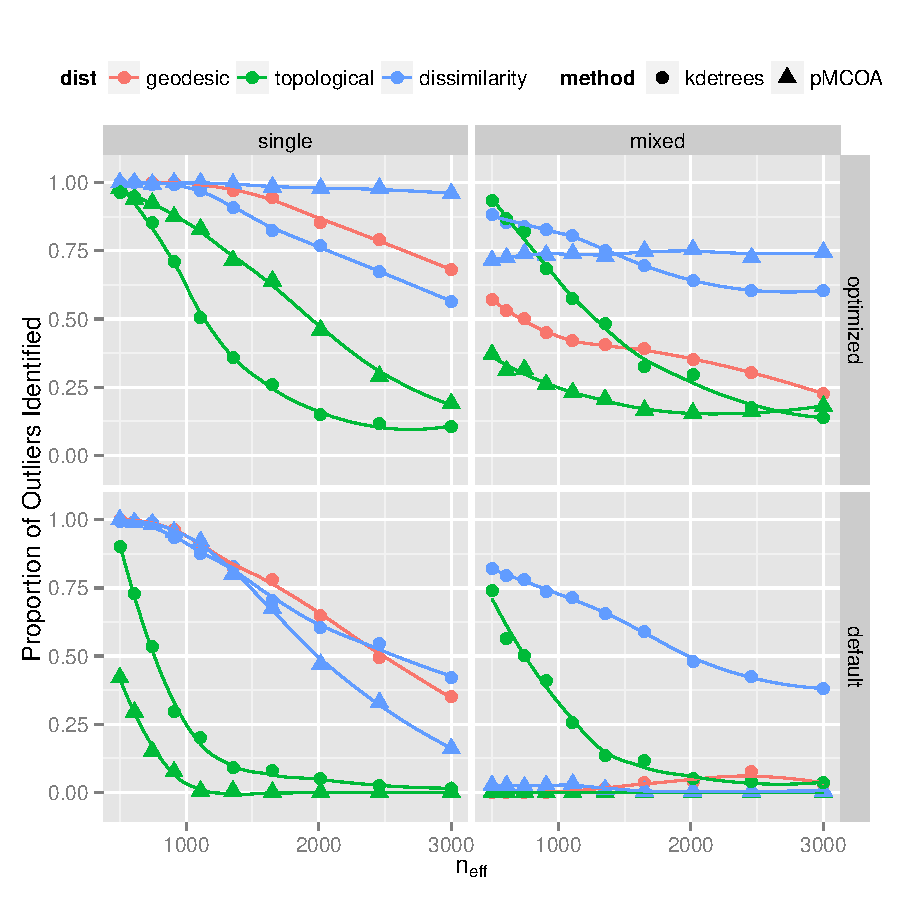
\includegraphics{img/tpr}
  \caption{Outlier identification rates.}
  \label{fig:tprplot}
\end{figure}


\begin{Schunk}
\begin{Sinput}
> library(phangorn)
> x <- replicate(10000,rtree(50),simplify=FALSE)
> class(x) <- "multiPhylo"
> timing <- function(i,fn,...) system.time(fn(x[1:i],...))
> foo <- function(x) aggregate(time~expr,x,mean)
> n <- floor(10^seq(1,3.699,length.out=10))
> kdebench3 <- sapply(n,timing,kdetrees,distance="d")
> pmcbench3 <- sapply(n,timing,pmcoa)
> save(kdebench3,pmcbench3,file="sim/bench.Rda")
\end{Sinput}
\end{Schunk}

\begin{Schunk}
\begin{Sinput}
> foo <- function(x) data.frame(n=n,time=ISOdate(2001,1,1,0)+as.data.frame(t(x))$elapsed,method=as.character(match.call()[[2]]))
> bench.df <- rbind(foo(kdebench3),foo(pmcbench3))
> ggplot(bench.df,aes(x=n,y=time,pch=method))+geom_point(size=3)+labs(y="hours")+theme(legend.position="top")+scale_x_continuous(limits=c(500,5000))
> ggsave("img/bench.pdf",height=3,width=7)
\end{Sinput}
\end{Schunk}

\begin{figure}
  \centering
  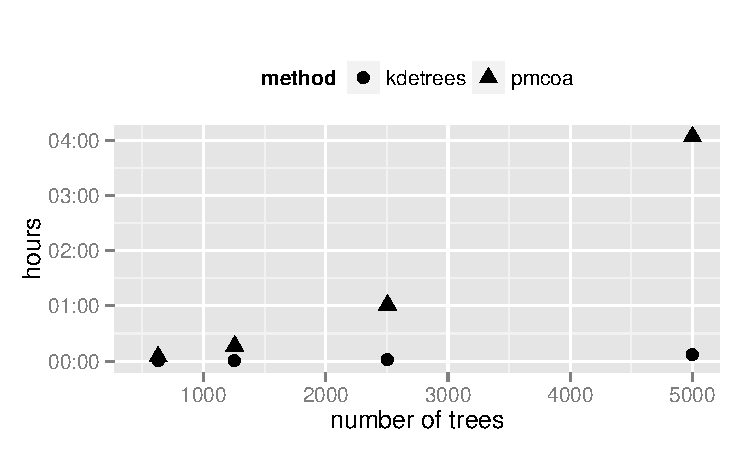
\includegraphics{img/bench}
  \caption{Benchmarks}
  \label{fig:bench}
\end{figure}

\begin{Schunk}
\begin{Sinput}
> #ggplot(sim1.res,aes(neff,values,color=Method,shape=Method,linetype=Distance)) + facet_grid(.~model) + theme(legend.position="top",legend.box="horizontal") + coord_trans("log") + stat_smooth(se=FALSE,method="loess",span=.99) + geom_point(size=2.5) + labs(title="Outliers Identified",x="Effective Population Size",y="Proportion of simulations") + scale_color_brewer(type="qual",palette=2) + scale_x_continuous(breaks=c(500,1000,1500,2000,3000)) + scale_color_grey(end=0.5)
\end{Sinput}
\end{Schunk}


\end{document}
